% !TeX root = RJwrapper.tex
\title{gplsim: An R Package for Generalized Partially Linear Single-index Models}
\author{by Tianhai Zu and Yan Yu}

\maketitle

\abstract{
  Generalized partially linear single-index models (GPLSIMs) are important tools in nonparametric regression. They extend popular generalized linear models to allow flexible nonlinear dependence on some predictors while overcoming the ``curse of dimensionality.'' We develop an R package \pkg{gplsim} that implements efficient spline estimation of GPLSIMs, proposed by \cite{yu_penalized_2002} and \cite{yu_penalised_2017}, for a response variable from a general exponential family. The package builds upon the popular \pkg{mgcv} package for generalized additive models (GAMs) and provides functions that allow users to fit GPLSIMs with various link functions, select smoothing tuning parameter $\lambda$ against generalized cross-validation or alternative choices, and visualize the estimated unknown univariate function of single-index term. In this paper, we discuss the implementation of \pkg{gplsim} in detail, and illustrate the use case through a sine-bump simulation study with various links and a real-data application to air pollution data.
}

\section{Introduction}

A popular approach to analyzing the relationship between a response variable and a set of predictors is generalized linear models or GLMs \cite{mccullagh_generalized_1989}, where the conditional mean of the response variable is linked to a linear combination of predictors via a link function. Although GLMs are simple and easy to interpret, in many complex real data applications the underlying assumption of linearity is often violated. Generalized partially linear single-index models (GPLSIMs) \citep[e.g.][]{carroll_generalized_1997,yu_penalized_2002,yu_penalised_2017} are flexible semiparametric models that allow for a non-linear relationship while retaining ease of interpretation. In particular, GPLSIMs include a partial linear component $\mathbf{z} \boldsymbol{\gamma}$, and importantly a nonparametric single-index component, effectively reducing the dimensionality of $p$-dimensional predictors $\mathbf{x}$ to a univariate single index $\mathbf{x}^{T} \boldsymbol{\theta}$ with a flexible univariate function $\phi(\mathbf{x}^{T} \boldsymbol{\theta})$, avoiding the ``curse of dimensionality" in multivariate nonparametric regression. GPLSIMs reduce to popular single-index models \citep{ichimura_semiparametric_1993,hardle_optimal_1993,xia_semi-parametric_2006} when there are no partial linear terms. Another popular special case is partially linear models \cite{hardle_partially_2012} when there is only one predictor in the nonparametric component.

GPLSIMs and the reduced models have been studied extensively in the literature. Applications lie in various fields, for example, discrete choice analysis, dose-response models, credit scoring, Framingham heart study \citep[][and references therein]{yu_penalised_2017}.  
\cite{yu_penalized_2002}, \cite{xia_semi-parametric_2006}, and \cite{liang_estimation_2010} studied partially linear single-index models for continuous responses. For responses from a general exponential family, \cite{carroll_generalized_1997} proposed local linear approach via quasi-likelihood for GPLSIMs estimation. 
However, as noted in \cite{yu_penalized_2002}, the algorithm using local linear methods in \cite{carroll_generalized_1997} may suffer from some computational issues and can become unstable. \cite{yu_penalized_2002} proposed a stable and computationally expedient approach using penalized splines (P-splines) with non-linear least square minimization. \cite{yu_penalised_2017} further proposed an efficient profile likelihood algorithm for the P-splines approach to GPLSIMs. 

We develop a package \pkg{gplsim}\footnote{The package has been published at CRAN, and it is hosted at the package maintainer's public GitHub repository \url{github.com/zzz1990771/gplsim}.} in R \citep{R2021} using splines for efficient estimation of the unknown univariate function in GPLSIMs following \cite{yu_penalized_2002} and \cite{yu_penalised_2017}. The \pkg{gplsim} R package mainly implements the profile likelihood estimation method described in \cite{yu_penalised_2017}, utilizing the function \code{gam} \citep{Wood_fast_2011} from the state-of-the-art R package \pkg{mgcv} \citep{wood_mgcv_2001}. The model class \code{gplsim} extends on the \code{gam} for straightforward computation and implementation. A side benefit is that our \pkg{gplsim} package enjoys improvements and features as those made to the \pkg{mgcv} package. For example, \pkg{mgcv 1.5} added smoothness selection method ``REML'' and ``ML'' in addition to ``GCV'' to its core function ``gam()'', and \pkg{gplsim} can enjoy those new features naturally. Similarly, any spline basis adopted in \pkg{mgcv} package, such as the thin plate regression spline basis, is also available in our \pkg{gplsim} package. In addition, our \pkg{gplsim} package also implements the simultaneous non-linear least square minimization methods for continuous responses from \cite{yu_penalized_2002} as an alternative option. 

The \pkg{mgcv} package for generalized additive models (GAMs) is indeed a fundamental building block for our \pkg{gplsim} package. GAMs \citep{Hastie1986,Wood_fast_2011} are popular semiparametric models, which replaces the single-index components by summation of individual smooth functions. As noted in \citet{carroll_generalized_1997} and \citet{yu_penalized_2002}, GPLSIMs are more parsimonious and can model some interactions. However, GPLSIMs are nonlinear and more difficult to estimate, especially given the widely available software for GAMs. One may view GAMs as a special case of GPLSIMs when the single-index coefficients are known. Alternatively, one may view GPLSIMs as special GAMs models with a nonlinear single-index effect. Single-index models can also be viewed as the base of more complex models, such as multi-index models \citep{xia_multiple_index_2008}, projection pursuit regression \citep{hall_projection_1989} and deep neural networks \citep{yang_high_dimensional_2017}. 

The rest of the paper is organized as follows. In the next section, we review the GPLSIMs and the penalized spline estimation for GPLSIMs. Next, we discuss the estimation algorithm implemented in this package. The following section describes the main features of the functions provided. The section ``real data and simulation examples'' illustrates the use of \pkg{gplsim} in R via an air pollution example and a sine-bump simulation study. The last section summarizes the method and presents directions for future research and application.

\section{An overview of generalized partially linear single-index models}

\subsection{The GPLSIMs}

For given predictor vectors of $p$-dimensional $X=\mathbf{x}$ and $q$-dimensional $Z=\mathbf{z}$, and under the assumption that the conditional density of the response variable $Y$ arises from a general exponential family, the conditional mean $E(Y|\mathbf{x}, \mathbf{z})$ can be modeled by 
\begin{equation}
  E(Y|\mathbf{x}, \mathbf{z}): = \mu(\mathbf{x}, \mathbf{z}) = g^{-1}\{\phi\left(\mathbf{x}^{T} \boldsymbol{\theta}\right)+\mathbf{z} \gamma\},
 \label{eq:GPLSIM} 
\end{equation}
where the single-index parameter $\boldsymbol{\theta}$ maps the $p$-dimensional predictors $\mathbf{x}$ to a univariate single index $\mathbf{x}^{T} \boldsymbol{\theta}$ by a linear projection, and $\phi(\cdot)$ is a univariate unknown function, while $g\{\cdot\}$ is a known link function. The parameter vector is constrained such that $\left\|\boldsymbol{\theta}\right\|=1$ with first element $\theta_1$ positive for identifiability \citep{yu_penalized_2002}. 
%This constraint can be handled by reparameterizing $\boldsymbol{\theta}=\left(1, \boldsymbol{\zeta}\right) / \sqrt{1+\|\boldsymbol{\zeta}\|^{2}}$ where $\zeta$ is an unconstrained parameter vector with one dimension lower than $\boldsymbol{\theta}$. 

One of the main challenges to estimate model~(\ref{eq:GPLSIM}) is that the $p$-dimensional single-index parameter $\boldsymbol{\theta}$ is nested within the unknown univariate function $\phi(\cdot)$, and hence a highly nonlinear problem.

\subsection{Review of penalized spline estimation for GPLSIMs}

When the single-index parameter $\boldsymbol{\theta}$ or the single-index $u=\mathbf{x}^{T} \boldsymbol{\theta}$ is given,  we can estimate the unknown univariate function $\phi(\cdot)$ with penalized splines \citep{ruppert2003semiparametric} such that $\phi(u) \approx \mathbf{H}(u)\boldsymbol{\beta}$. The systematic component of GPLSIMs can then be approximated by
\begin{equation}g\{\mu(\mathbf{x}, \mathbf{z})\}=\mathbf{H}(\mathbf{x}^{T} \boldsymbol{\theta}) \boldsymbol{\beta}+\mathbf{z} \boldsymbol{\gamma},
\end{equation}
where $\mathbf{H}(\cdot)$ is the spline basis, and $\boldsymbol{\beta}$ is the spline coefficient vector. We denote $\boldsymbol{\omega}=\left(\boldsymbol{\theta}, \boldsymbol{\beta}, \boldsymbol{\gamma}\right)$ as the column parameter vector.

There are many choices of the spline basis functions $\mathbf{H}({\cdot})$, such as B-spline, truncated power basis, thin-plate spline, and their variations. For simplicity, we first illustrate using a truncated power basis of degree $d$: 
$$
\begin{aligned}
  \mathbf{H}(u) \boldsymbol{\beta} =\beta_{0}+\beta_{1} u+\cdots+\beta_{d} u^{d}+\sum_{k=1}^{K} \beta_{d+k}\left(u-v_{k}\right)_{+}^{d}, 
  \end{aligned}
$$  
where $\mathbf{H}(u)=\left\{1, u, \ldots, u^{d},\left(u-v_{1}\right)_{+}^{d}, \ldots,\left(u-v_{K}\right)_{+}^{d}\right\}$ are spline bases with $K$ interior knots placed at $\left(v_{1}, \ldots, v_{K}\right)$. Quadratic or cubic splines are commonly used. The interior knots are usually placed at equally-spaced quantiles within the domain.

Another popular choice of spline basis is the B-spline basis. Any B-spline basis functions $\mathbf{H}({\cdot})$ of degree higher than 0, can be defined by the following Cox-de Boor recursion formula \citep{boor_practical_2001}: 
$$
  \mathrm{H}_{k, \mathrm{d}}(u)=\frac{u-u_{k}}{u_{k+d-1}-u_{k}} \mathrm{H}_{k, d-1}(u)+\frac{u_{k+d}-u}{u_{k+d}-u_{k+1}} \mathrm{H}_{k+1, d-1}(u),
$$
where
$$
  \mathrm{H}_{k, 0}(u)=\left\{\begin{array}{ll}
  1, & \mathrm{u}_{k} \leq u \leq u_{k+1} \\
  0, & \text { otherwise. }
  \end{array}\right.
$$
One of the appealing features of the B-spline is that, unlike truncated power basis, B-spline basis functions have local supports that can result in high numerical stability.

To avoid overfitting, a roughness penalty controlled by a smoothing parameter $\lambda$ is applied to the log-likelihood. Specifically, we can obtain the penalized log-likelihood estimator of $\boldsymbol{\omega}$ by maximizing the following penalized log-likelihood function:
\begin{equation}\begin{aligned}
  Q_{n, \lambda}(\boldsymbol{\omega})=& \frac{1}{n} L_{n}(\boldsymbol{\omega})-\frac{1}{2} \lambda \boldsymbol{\beta}^{\top} \mathbf{D} \boldsymbol{\beta} \\
  =& \frac{1}{n} \sum_{i=1}^{n}\left[y_{i} \xi\left(\mathbf{x}_{i}, \mathbf{z}_{i} ; \boldsymbol{\omega}\right)-b\left\{\xi\left(\mathbf{x}_{i}, \mathbf{z}_{i} ; \boldsymbol{\omega}\right)\right\}\right] -\frac{1}{2} \lambda \boldsymbol{\beta}^{\top} \mathbf{D} \boldsymbol{\beta},
 \label{eq:plike}
\end{aligned}\end{equation}
where $\xi$ is the natural parameter in generalized linear models, $\mu(\mathbf{x}_{i}, \mathbf{z}_{i})  = b^{\prime}\left\{\xi\left(\mathbf{x}_{i}, \mathbf{z}_{i} ; \boldsymbol{\omega}\right)\right\}$, for observations $i=1,\cdots,n$, and $\mathbf{D}$ is a positive semidefinite symmetric penalty matrix. Common penalty matrices include the usual quadratic integral penalty on second derivatives of $\phi(\cdot)$ or alternatively the diagonal penalty matrix with its last $K$ diagonal elements constrained to equal to one and the rest equal to zero \citep[see e.g.][]{ruppert_theory_2000,yu_penalized_2002}, which in effect penalizes the coefficients of the truncated power basis at the jump of $d$-th derivatives. 

Maximizing the penalized log-likelihood function~(\ref{eq:plike}) can be achieved in several ways. We mainly focus on implementing an efficient profile log-likelihood method in \cite{yu_penalised_2017}. We also present an option to implement a simultaneous nonlinear least square method in \cite{yu_penalized_2002}. 

The selection of smoothing parameter $\lambda$ is important as it controls the tradeoff between over-smoothing (possible underfitting) and under-smoothing (possible overfitting). We use an outer iteration to select $\lambda$ against some selection criterion, as recommended by \cite{Wood_fast_2011}. For the default choice, we adopt generalized cross validation (GCV) to select the smoothing parameter $\lambda$. Alternatively, we can consider maximum likelihood (ML) \citep{anderssen_time_1974} or restricted maximum likelihood (REML) \citep{wahba_comparison_1985} based approaches. A nice feature is that we can directly adopt criteria that have been provided by the ``gam()'' function arguments from R package \pkg{mgcv}, which is one of the main components in the implementation of our \code{gplsim} estimation algorithm. 

\subsection{Algorithm}

We present the main algorithm for fitting the generalized partially linear single-index models (GPLSIMs) with penalized splines estimation with profile likelihood in detail as follows: 

\begin{algorithm}[H]  
  \KwIn{Non-linear predictor vector of $p$-dimensional $X=\mathbf{x}$, partially linear predictor vector of $q$-dimensional $Z=\mathbf{z}$, and a response vector $Y=\mathbf{y}$ of family=family.}
  \KwOut{The estimated single-index parameter $\widehat{\boldsymbol{\theta}}$, spline coefficient $\widehat{\boldsymbol{\beta}}$, partially linear coefficient $\widehat{\boldsymbol{\gamma}}$, and fitted response $\widehat{\mathbf{y}}$.}

  Obtain an initial estimate $\hat{\boldsymbol{\theta}}^{(0)}$ of the single-index parameter $\boldsymbol{\theta}$ from a generalized linear model (default), or a user-provided initial list.

  With an estimate of ${\boldsymbol{\theta}}$ (equivalently, the single index $\left\{u_{i}=\mathbf{x}^{T}_{i} {\boldsymbol{\theta}}: i=1, \ldots, n\right\}$ ), the spline coefficient ${\boldsymbol{\beta}}$ and partially linear coefficient ${\boldsymbol{\gamma}}$ can be written as implicit functions of ${\boldsymbol{\theta}}$ to maximize penalized log-likelihood:
  \begin{equation*}\begin{array}{l}
    Q\left(\boldsymbol{\beta}, \boldsymbol{\gamma}, \lambda ; u_{1}, \ldots, u_{n}\right) \\
    =\frac{1}{n} \sum_{i=1}^{n}\left[y_{i} \xi\left(u_{i}, \mathbf{z}_{i} ; \boldsymbol{\beta}, \boldsymbol{\gamma}\right)-b\left\{\xi\left(u_{i}, \mathbf{z}_{i} ; \boldsymbol{\beta}, \boldsymbol{\gamma}\right)\right\}\right] \\
    \quad-\frac{1}{2} \lambda \boldsymbol{\beta}^{\top} \mathbf{D} \boldsymbol{\beta}.
    \end{array}\end{equation*}
   The roughness penalty parameter $\lambda$ is selected using generalized cross-validation score (default) or alternative options.

  Given the spline coefficient vector $\widehat{\boldsymbol{\beta}}_{\lambda}(\boldsymbol{\theta})$ and partially linear coefficient vector $\widehat{\boldsymbol{\gamma}}_{\lambda}(\boldsymbol{\theta})$ as implicit functions of
  ${\boldsymbol{\theta}}$, obtain the profile log-likelihood estimator of the single-index parameter $\boldsymbol{\theta}$ by maximizing:
  \begin{equation*}
  \begin{aligned}
    Q(\boldsymbol{\theta})=& \frac{1}{n} \sum_{i=1}^{n}\left[y_{i} \xi\left(\mathbf{x}^{T}_{i} \boldsymbol{\theta}, \mathbf{z}_{i} ; \widehat{\boldsymbol{\beta}}_{\lambda}(\boldsymbol{\theta}), \widehat{\boldsymbol{\gamma}}_{\lambda}(\boldsymbol{\theta})\right)\right.\\
    &\left.-b\left\{\xi\left(\mathbf{x}^{T}_{i} \boldsymbol{\theta}, \mathbf{z}_{i} ; \widehat{\boldsymbol{\beta}}_{\lambda}(\boldsymbol{\theta}), \widehat{\boldsymbol{\gamma}}_{\lambda}(\boldsymbol{\theta})\right)\right\}\right].
  \end{aligned}
  \end{equation*}

  With the estimated profile log-likelihood estimator $\widehat{\boldsymbol{\theta}}$ of the single-index parameter, obtain the final estimator $\widehat{\boldsymbol{\beta}}$ of spline coefficient and $\widehat{\boldsymbol{\gamma}}$ of partially linear coefficient via step 2.

  Obtain the final fitted response vector $\widehat{\mathbf{y}}$ from model~(\ref{eq:GPLSIM}). 

\end{algorithm}

Alternatively, for continuous responses under the default assumption of $family=gaussian$, maximizing the penalized log-likelihood estimator equation~(\ref{eq:plike}) is equivalent to minimizing the penalized sum of squared errors:
\begin{equation*}\begin{aligned}
\frac{1}{n} \sum_{i=1}^{n}\left\{y_{i} - \mathbf{H}(\mathbf{x}^{T}_{i} \boldsymbol{\theta}) \boldsymbol{\beta} - \mathbf{z}_{i}\boldsymbol{\gamma}\right\}^{2} + \frac{1}{2} \lambda \boldsymbol{\beta}^{\top} \mathbf{D} \boldsymbol{\beta}.
\end{aligned}\end{equation*}
For the simultaneous non-linear least square minimization methods in \cite{yu_penalized_2002}, we can directly apply a standard nonlinear least square  (NLS) optimization algorithm on minimization of the above penalized sum of squared errors with respect to the full parameter $\boldsymbol{\omega}=\left(\boldsymbol{\theta}, \boldsymbol{\beta}, \boldsymbol{\gamma}\right)$. This is useful to facilitate joint inferences as described in \cite{yu_penalized_2002}. This algorithm as presented in \cite{yu_penalized_2002} is also implemented in our \pkg{gplsim} package.

{\bf Remark.} In Step 2 of the profile-likelihood algorithm implementing \cite{yu_penalised_2017} as well as the simultaneous non-linear least square minimization methods implementing \cite{yu_penalized_2002}, the spline knots used for the basis functions depend on  $\boldsymbol{\theta}$ because they are sample quantiles or equally-spaced placed on the single index $\{\boldsymbol{x}^{T}_{i} \boldsymbol{\theta}, i=1,...,n\}.$ That is, the spline coefficient ${\boldsymbol{\beta}}$, along with the spline knots implicitly, depends on the single index coefficient ${\boldsymbol{\theta}}$. We refer to the original methodological papers \cite{yu_penalized_2002}, \cite{yu_penalised_2017}, and references therein for more details.

%However, when the parameter dimension gets larger, the simultaneous NLS algorithm is less desirable than an iterative algorithm by essentially iterating step 2 and step 3 until convergence, where
%$Q\left(\cdot\right)$ in step 2 is equivalent to minimizing the penalized sum of squared errors:
%\begin{equation*}\begin{array}{l}
%Q\left(\boldsymbol{\beta}, \boldsymbol{\gamma}, \lambda ; u_{1}, \ldots, u_{n}\right) \\
%=\frac{1}{n} \sum_{i=1}^{n}\left\{y_{i} - \mathbf{H}(u_i) \boldsymbol{\beta} - \mathbf{z}_{i}\boldsymbol{\gamma}\right\}^{2} + \frac{1}{2} \lambda \boldsymbol{\beta}^{\top} \mathbf{D} \boldsymbol{\beta}.
%\end{array}\end{equation*}
%These algorithms as presented in \cite{yu_penalized_2002} are also implemented in our \pkg{gplsim} package.

\section{The gplsim package}
The R package \pkg{gplsim} consists of one core estimation function \code{gplsim} and some supporting functions such as visualization of the estimated curve for the unknown univariate function. The R package \pkg{gplsim} depends on the R package \pkg{mgcv} \citep{wood_mgcv_2001} and package \pkg{minpack.lm} \citep{minpack2022}. Unit tests using \pkg{testthat} are in place to ensure continued robustness of the package.

\subsection{Main fitting function}

The main estimation function \code{gplsim} implements the profile likelihood algorithm of \cite{yu_penalised_2017} as well as the non-linear least square method of \cite{yu_penalized_2002} described in the previous section. The default method is the profile likelihood for responses from a general exponential family and non-linear least square method for others. 

The usage and input arguments of the main fitting function \code{gplsim} are summarized as follows:

\begin{example}
  gplsim(Y, X, Z, family = gaussian, penalty = TRUE, profile = TRUE, user.init = NULL,
   bs= "ps", ...)
\end{example}

This function takes three required arguments: the response variable $Y$ in vector format, the single-index nonlinear predictors $X$ in the matrix or vector format, and the linear predictors $Z$ in the matrix or vector format. Please note that all the input covariates are required to be numeric variables. 

This function also takes several optional arguments for finer controls. The optional argument \code{family} is a family object for models from the built-in R package \pkg{stats}. This object is a list of functions and expressions for defining link and variance functions. Supported link functions include identity; logit, probit, cloglog; log; and inverse for the family distributions of Gaussian, Binomial, Poisson, and Gamma, respectively. Other families supported by \code{glm} and \code{mgcv::gam} are also supported. The optional argument \code{penalty} is a logical variable to specify whether to use penalized splines or un-penalized splines to fit the model. The default value is TRUE to implement penalized splines. The optional argument \code{profile} is a logical variable that indicates whether the algorithm with profile likelihood or the algorithm with NLS procedure is used. The default algorithm is set to the profile likelihood algorithm. The optional argument \code{user.init} is a numeric vector of the same length as the dimensionality of single-index predictors. The users can use this argument to pass in any appropriate user-defined initial single-index coefficients based on prior information or domain knowledge. The default value is NULL, which instructs the function to estimate initial single-index coefficients by a generalized linear model.


 As we utilize \code{mgcv::gam} and \code{mgcv::s} as the underlying algorithms for the estimation of the unknown univariate function of the single index, there are several arguments that can be passed into \code{mgcv::gam} and \code{mgcv::s} for finer control. For example, the optional argument \code{bs} is a character variable that specifies the spline basis in the estimation of the single index function, and it will be passed into \code{mgcv::s}. The default has been set to ``ps'' (P-splines with B-spline basis) while other choices are ``tr'' (truncated power basis), ``tp'' (thin plate regression splines), and others (see the help page of \code{mgcv::smooth.terms}). Other \code{mgcv::gam} arguments can be passed to \code{mgcv::s} in \code{...} includes the optional numeric arguments \code{k}, which is the dimension of the basis of the smooth terms and the arguments \code{m}, which is the order of the penalty for the smooth terms. Additionally, users can also pass arguments \code{scale} into \code{gam} in \code{...}. It is a numeric indicator with a default value set to -1. Any negative value including -1 indicates that the scale of response distribution is unknown and thus needs to be estimated. Another option is 0, indicating a scale of 1 for Poisson and binomial distribution and unknown for others. Any positive value will be taken as the known scale parameter. The optional argument \code{smoothing\_selection} is a character variable that specifies the criterion used in the selection of the smoothing parameter $\lambda$. This argument corresponds to the argument \code{method} in \code{mgcv::gam}, but it is renamed in this package to avoid confusion. The supported criteria include ``GCV.Cp'',``GACV.Cp'', ``ML'',``P-ML'', ``P-REML'' and ``REML'', while the default criterion is ``GCV.Cp''. For more details regarding arguments in \code{mgcv::gam} and \code{mgcv::s}, users may refer to the help page of \code{mgcv::gam} and \code{mgcv::s}.

The function \code{gplsim} returns an object class of \code{gplsim}, which extends the \code{gam} object and \code{glm} object.

\subsection{Other functions}

\begin{example}
  plot_si(gplsim.object,reference = NULL)
\end{example}
This function plots the estimated curve for the unknown univariate function $\phi$ from a gplsim-fitted model object. If the reference object is provided, this function will add a reference line accordingly. 


\begin{example}
  summary.gplsim(gplsim.object)
  print.summary.gplsim(gplsim.object)
\end{example}

The functions \code{summary.gplsim} and \code{print.summary.gplsim} provide detailed information related to the fitted model and summarize the results as illustrated in the next section. These two functions can be called directly by applying functions print and summary to gplsim.object. 

\begin{example}
  simulation_data <- generate_data(n,true.beta=c(1, 1, 1)/sqrt(3),family="gaussian")
\end{example}

The function \code{generate\_data} generates data from a sine-bump model with user-defined single index coefficients $\boldsymbol{\theta}$ via the argument \code{true.beta}. If single-index coefficients $\boldsymbol{\theta}$ are not provided, this function will generate data against the default coefficients $\boldsymbol{\theta} = (1,1,1) / \sqrt{3}$. The default response is Gaussian distributed, while Binomial, Poisson, and Gamma distributions are also supported.

\section{Real data and simulation examples}

In this section, we demonstrate the use of the R package \pkg{gplsim} via a real data analysis and a sine-bump simulation study. 


\subsection{Air Pollution Data}\label{air-pollution-data}
  
We consider an environmental study on how meteorological variables $X$ affect the concentration of the air pollutant ozone $y$. Meteorological variables $X$ contain wind speed, temperature, and radiation with $n=111$ daily measurements. As the response variable $y$ is a continuous variable, we adopt an identity link for Gaussian distribution. Note that we use the same sequence of predictor variables to keep the results directly comparable to \cite{yu_penalized_2002}.

\begin{Schunk}
  \begin{Sinput}
  library(gplsim)
  data(air)
  y=air$ozone                    # response
  X=as.matrix(air[,c(3,4,2)])    # single-index term
  colnames(X)=colnames(air[,c(3,4,2)])
  Z=NULL
  \end{Sinput}
\end{Schunk}

We allow all three predictor variables, temperature, wind speed, and radiation, to enter the single-index term to capture the non-linear dependency as in \cite{yu_penalized_2002}. This model collapses to the single-index model as there is no partially linear term in the model.

\begin{Schunk}
  \begin{Sinput}
  air.fit <- gplsim(y,X,Z=NULL,family = gaussian,bs="ps")
  summary(air.fit)
  \end{Sinput}
  \begin{Soutput}
  #> 
  #> Family: gaussian 
  #> Link function: identity 
  #> 
  #> Formula:
  #> y ~ s(a, bs = bs, fx = fx, m = 2, k = k)
  #> 
  #> partial linear coefficients:
  #>           Estimate Std. Error t value  Pr(>|t|)    
  #> Intercept 3.247784   0.043024  75.488 < 2.2e-16 ***
  #> ---
  #> Signif. codes:  0 '***' 0.001 '**' 0.01 '*' 0.05 '.' 0.1 ' ' 1
  #> 
  #> 
  #> single index coefficients:
  #>             Estimate
  #> temperature   0.5442
  #> wind_speed   -0.8386
  #> radiation     0.0223
  #> 
  #> Approximate significance of smooth terms:
  #>         edf Ref.df      F   p-value    
  #> s(a) 8.1431  9.173 34.867 < 2.2e-16 ***
  #> ---
  #> Signif. codes:  0 '***' 0.001 '**' 0.01 '*' 0.05 '.' 0.1 ' ' 1
  #> 
  #> R-sq.(adj) =  0.741   Deviance explained =   76%
  #> GCV = 0.22391  Scale est. = 0.20546   n = 111
  \end{Soutput}
  \end{Schunk}

  The estimated normalized single-index coefficients with the profile likelihood algorithm are comparable to the results in \cite{yu_penalized_2002}. 
  As shown in the figure below, the estimated unknown function is quite monotonic and exhibits clear curvature. The estimated coefficient is positive for temperature, negative for wind speed, and positive for radiation but in a smaller magnitude per the reported summary. 

\begin{Schunk}
  \begin{Sinput}
  plot_si(air.fit,yscale=c(1,6),plot_data = TRUE)
  \end{Sinput}

  \begin{figure}[ht]
    \centering
    \addtolength{\leftskip} {-2cm}
    \addtolength{\rightskip}{-2cm}
    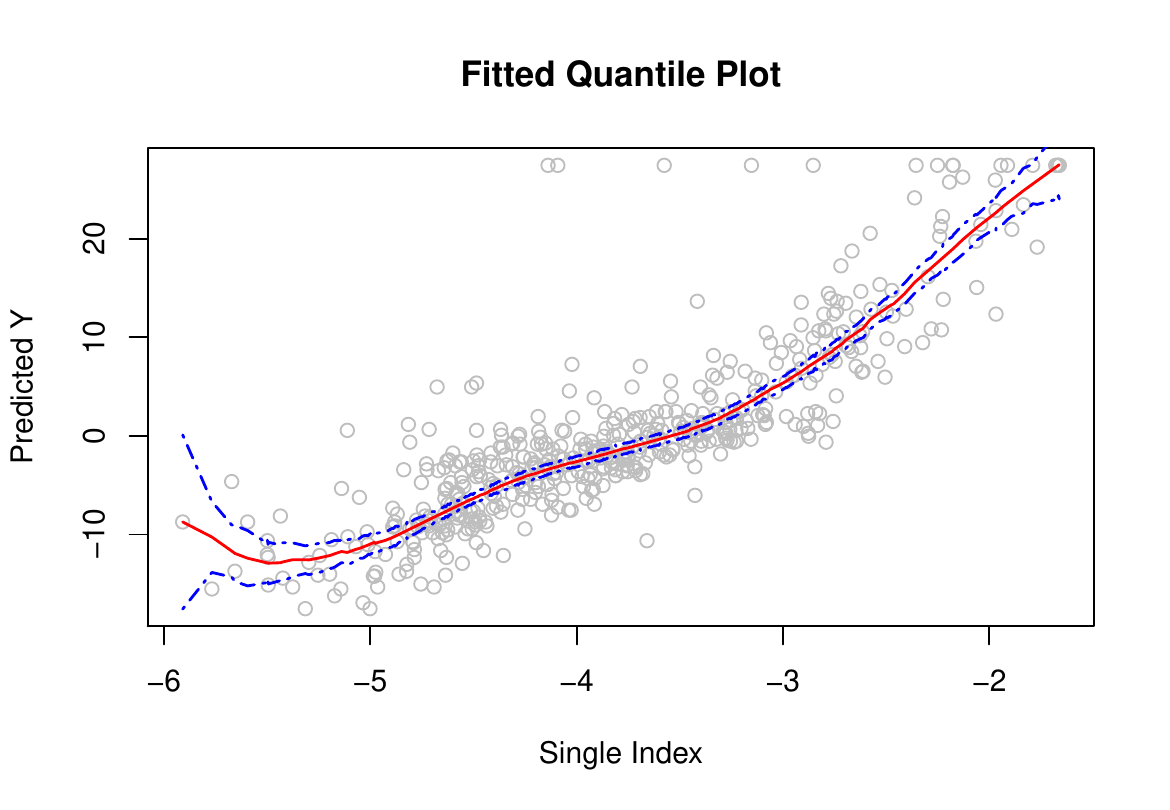
\includegraphics[width=9cm]{gplsim_files/figure-latex/unnamed-chunk-3-1} 
    \caption{Single-index curve estimate of the air pollution data, an output of function \code{plot\_si}. The data are represented
    	by dots.}
  \end{figure}
\end{Schunk}

The above figure shows the single-index curve estimate of the air pollution data. The presence of curvature with multiple turning points is observed. This non-linear dependency is unlikely to be captured by a linear model. The single index that contains information from temperature, wind speed, and radiation contributes to the ozone concentration differently in different segments. 

We also implemented the simultaneous non-linear least square minimization algorithm described in \cite{yu_penalized_2002}, where the original code was written in Matlab. 

\begin{Schunk}
  \begin{Sinput}
  air.fit <- gplsim(y,X,Z=Z,family = gaussian,profile = FALSE,bs="ps")
  summary(air.fit)
  \end{Sinput}
  \begin{Soutput}
  #> 
  #> Family: gaussian 
  #> Link function: identity 
  #> 
  #> Formula:
  #> y ~ s(a, bs = bs, fx = !penalty, m = 2, k = 13)
  #> 
  #> partial linear coefficients:
  #>           Estimate Std. Error t value  Pr(>|t|)    
  #> Intercept 3.247784   0.043056  75.431 < 2.2e-16 ***
  #> ---
  #> Signif. codes:  0 '***' 0.001 '**' 0.01 '*' 0.05 '.' 0.1 ' ' 1
  #> 
  #> 
  #> single index coefficients:
  #>             Estimate
  #> temperature   0.5340
  #> wind_speed   -0.8451
  #> radiation     0.0235
  #> 
  #> Approximate significance of smooth terms:
  #>         edf Ref.df     F   p-value    
  #> s(a) 8.0012 9.0533 35.22 < 2.2e-16 ***
  #> ---
  #> Signif. codes:  0 '***' 0.001 '**' 0.01 '*' 0.05 '.' 0.1 ' ' 1
  #> 
  #> R-sq.(adj) =   0.74   Deviance explained = 75.9%
  #> GCV = 0.22394  Scale est. = 0.20578   n = 111
  \end{Soutput}
\end{Schunk}

Note that here outputs are directly from mgcv package for GAM model summary. The p-value and confidence intervals here do not take into account the uncertainty in the estimation of the single-index coefficients. If required, valid inference using bootstrap or asymptotic results from \cite{yu_penalized_2002} and \cite{yu_penalised_2017} is available.


\subsection{Simulations}

We present a popular sine-bump simulation study that adopts the design as in \citep{carroll_generalized_1997, yu_penalised_2017, yu_penalized_2002}. The package can accommodate responses from a general exponential family, where the conditional mean is generated from the following model
\begin{equation*}
  g^{-1}\{\sin \left\{\pi\left(\mathbf{x}^{T} \boldsymbol{\theta}-c_{1}\right) /\left(c_{2}-c_{1}\right)\right\}+z \gamma\},
\end{equation*}
where $g\{\cdot\}$ is a link function$; \boldsymbol{\theta} = (1,1,1) / \sqrt{3}$ with each predictor $x$ from independent uniform in $[0,1]$; $\gamma=0.3$; $z$ is a binary predictor with $1$ for even observations and $0$ otherwise; $c_1= \sqrt{3}/2-1.645/\sqrt{12}$ and $c_2= \sqrt{3}/2+1.645/\sqrt{12}$ are two constants. 

For demonstration, we first show simulation codes and outputs on one random replication. We use the supporting function \code{generate\_data} to generate simulation data.
\begin{Schunk}
  \begin{Sinput}
  set.seed(2020)
  # Gaussian family
  # parameter settings
  n=1000
  M=200
  true.theta = c(1, 1, 1)/sqrt(3)
  # This function generates a sine-bump simulation data 
  data <- generate_data(n,true.theta=true.theta,family="gaussian",ncopy=M) 
  y=(data$Y)[[1]]       # Gaussian error with standard deviation 0.1
  X=data$X       # single-index predictors
  Z=data$Z       # partially linear predictors
  \end{Sinput}
  \end{Schunk}
  
We use default settings of the main estimation function \code{gplsim} on the simulated data, assuming no prior information. The codes and summary results are provided as follows.
\begin{Schunk}
  \begin{Sinput}
  result <- gplsim(y,X,Z,user.init=NULL,family = gaussian)
  summary(result)
  \end{Sinput}
  \begin{Soutput}
  #> 
  #> Family: gaussian 
  #> Link function: identity 
  #> 
  #> Formula:
  #> y ~ s(a, bs = bs, fx = fx, m = 2, k = k) + z
  #> 
  #> partial linear coefficients:
  #>            Estimate Std. Error t value  Pr(>|t|)    
  #> Intercept 0.6439549  0.0046579 138.251 < 2.2e-16 ***
  #> Z.1       0.3057685  0.0065963  46.354 < 2.2e-16 ***
  #> ---
  #> Signif. codes:  0 '***' 0.001 '**' 0.01 '*' 0.05 '.' 0.1 ' ' 1
  #> 
  #> 
  #> single index coefficients:
  #>     Estimate
  #> X.1   0.5786
  #> X.2   0.5798
  #> X.3   0.5736
  #> 
  #> Approximate significance of smooth terms:
  #>         edf Ref.df      F   p-value    
  #> s(a) 6.3561 7.4656 2129.9 < 2.2e-16 ***
  #> ---
  #> Signif. codes:  0 '***' 0.001 '**' 0.01 '*' 0.05 '.' 0.1 ' ' 1
  #> 
  #> R-sq.(adj) =  0.947   Deviance explained = 94.7%
  #> GCV = 0.010909  Scale est. = 0.010818  n = 1000
  \end{Soutput}
\end{Schunk}

From the above summary results of the fitted model, we see that the estimated single-index coefficients \(\widehat{\boldsymbol{\theta}}\) and partial-linear coefficients \(\widehat{\gamma}\) are quite close to the true parameters. 

We also plot the average estimated curve for the unknown univariate function over 200 replications. The dashed lines are the corresponding 2.5 and 97.5 quantiles bound. We observe that the average curve estimate virtually overlays the true curve. 

\begin{Schunk}
  \begin{Sinput}
  #plot the estimated univariate function curve
  plot_si(result,plot_data = FALSE)
  par(new=T)
  sort_index = order(X%*%true.theta)
  lines((X%*%true.theta)[sort_index],data$single_index_values[sort_index],lty=1,
  xaxt="n", yaxt="n",col="red")
  legend("topright",legend=c("GPLSIM fit", "True"),lty=c(1,1),col = c("black","red"))
  add_sim_bound(data)
  \end{Sinput}
  \begin{figure}[ht]
    \centering
    \addtolength{\leftskip} {-2cm}
    \addtolength{\rightskip}{-2cm}
    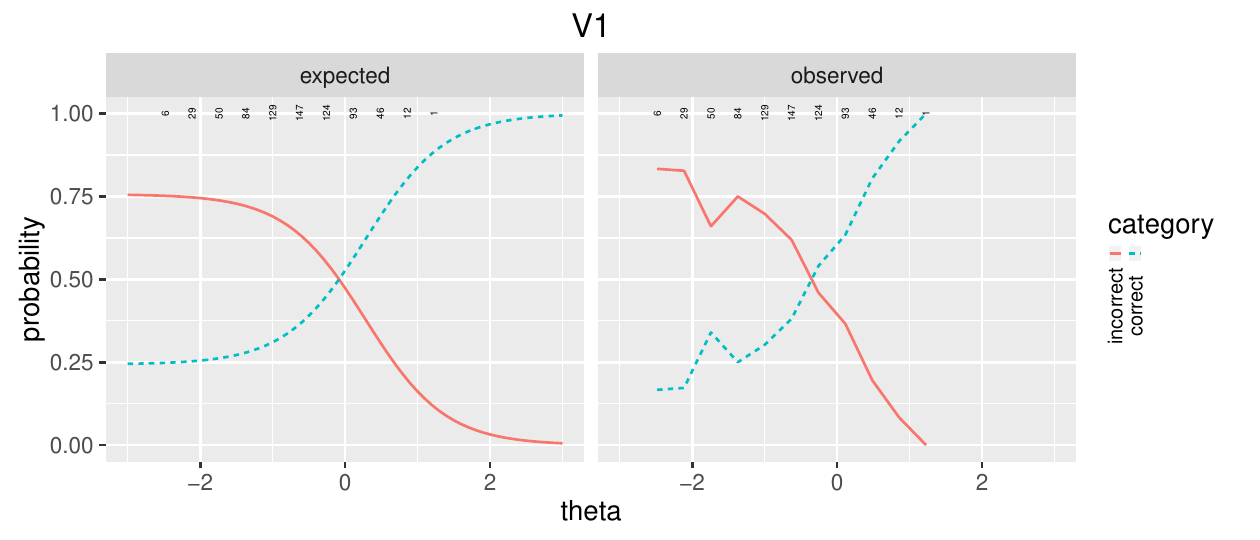
\includegraphics[width=10cm]{gplsim_files/figure-latex/unnamed-chunk-9-1}   
    \caption{
    Curve estimates and confidence bands for the unknown univariate function. The red
    solid curve is the true curve. The blue solid curve is
    the average fitted curve over 200 replications. The
    dashed curves are the corresponding $2.5\%$ and $97.5\%$
    quantiles.}
  \end{figure}
\end{Schunk}

Table~\ref{tb:sim} reports the mean, standard error (se) and bias for each parameter estimate with sample size $n=1000$ over $M=200$ replications. We use canonical link functions, that is, identity link for Gaussian family, logit link for Binomial family, and log link for Poisson family. One can see that the algorithm for our R package \pkg{gplsim} is effective in estimation of various GPLSIMs. 

\begin{table}[!ht]
	\centering
	\addtolength{\leftskip} {-2cm}
	\addtolength{\rightskip}{-2cm}
	
	\begin{tabular}{lllrllrllr}
    \toprule
		&  & \multicolumn{1}{r}{Gaussian} & \multicolumn{1}{c}{}     &  & \multicolumn{1}{r}{Binomial} & \multicolumn{1}{c}{}     &  & \multicolumn{1}{r}{Poisson}              & \multicolumn{1}{l}{}     \\ \cline{3-4} \cline{6-7} \cline{9-10} 
		&  & \multicolumn{1}{c}{Mean(se)} & \multicolumn{1}{c}{Bias} &  & \multicolumn{1}{c}{Mean(se)}         & \multicolumn{1}{c}{Bias} &  & \multicolumn{1}{c}{Mean(se)} & \multicolumn{1}{c}{Bias} \\ \hline
		$\hat{\theta}_1$ &  & 0.5771(0.0048)                      & -0.0002                  &  & 0.5545(0.1040)                       & -0.0228                  &  & 0.5808(0.0305)               & 0.0035                   \\
		$\hat{\theta}_2$ &  & 0.5774(0.0048)                      & 0.0005                   &  & 0.5744(0.1111)                       & -0.0029                  &  & 0.5738(0.0349)               & -0.0035                  \\
		$\hat{\theta}_3$ &  & 0.5765(0.0047)                      & -0.0004                  &  & 0.5717(0.1126)                       & -0.0056                  &  & 0.5745(0.0340)               & -0.0028                  \\
		$\hat{\gamma}$  &  & 0.2995(0.0065)                      & -0.0004                  &  & 0.3094(0.1312)                       & 0.0094                   &  & 0.2978(0.0430)               & -0.0022                 \\
    \toprule
  \end{tabular}
\caption{Summary of parameter estimates for various responses of sample size $n=1000$. True $\boldsymbol{\theta} = (1,1,1)/{\sqrt{3}}, \gamma = 0.3$. The sample mean (mean), standard error (se, in parenthesis), and bias of the parameter estimates from generalized partially linear single-index models (GPLSIMs) by penalized splines from 200 replications.}
\label{tb:sim}
\end{table}


  
\section{Summary}
In this paper, we have presented an R package \pkg{gplsim} that implements generalized partial linear single-index models described in \cite{yu_penalised_2017} and \cite{yu_penalized_2002}. The functions and algorithms used in the package are able to accurately estimate the single-index coefficients, partial-linear coefficients, as well as the unknown univariate function with expedient computation. We believe this package will be useful to practitioners in diverse fields such as finance, econometrics, and medicine, where a flexible and interpretable models are desirable. 

\newpage

\bibliography{gplsim} 


\address{Tianhai Zu\\
  The University of Texas at San Antonio\\
  One UTSA Circle \\
  San Antonio, TX 78249 \\
  https://orcid.org/0000-0002-4634-7937\\
  \email{tianhai.zu@utsa.edu}}

\address{Yan Yu\\
  University of Cincinnati\\
  2906 Woodside Drive\\
  Cincinnati, OH 45221 \\
  https://orcid.org/0000-0002-2859-3093\\
  \email{Yan.YU@uc.edu}}




